\section{Bitmap}

\subsection{Pourquoi le bitmap?}
Le format BITMAP aussi appelé DIB (Device Independent Bitmap) a été conçu par Windows corporation pour pouvoir échanger des images entre devices sans avoir à se soucier de la logique de ceux-ci.
Ces images ont des extensions .bmp ou encore .dib.
Techniquement, une image bitmap est un format de fichier non compressé, cela signifie entre autre que chaque pixel possède sa représentation sous forme d'un bit ou d'une série de bits.
On peut donc opposer sa structure à celle d'une image PNG, JPEG ou encore GIF qui utilise la compression pour regrouper des pixels similaires afin de réduire la taille globale du fichier.
On les appelle donc bitmaps car ils ne sont pas compressés (possible de le faire cependant).
Ils n'ont donc aucune perte de données et sont donc généralement plus lourds.\\
La structure du format BITMAP est connue et disponible en ligne. En voici un schéma :

\vspace{1.5cm}

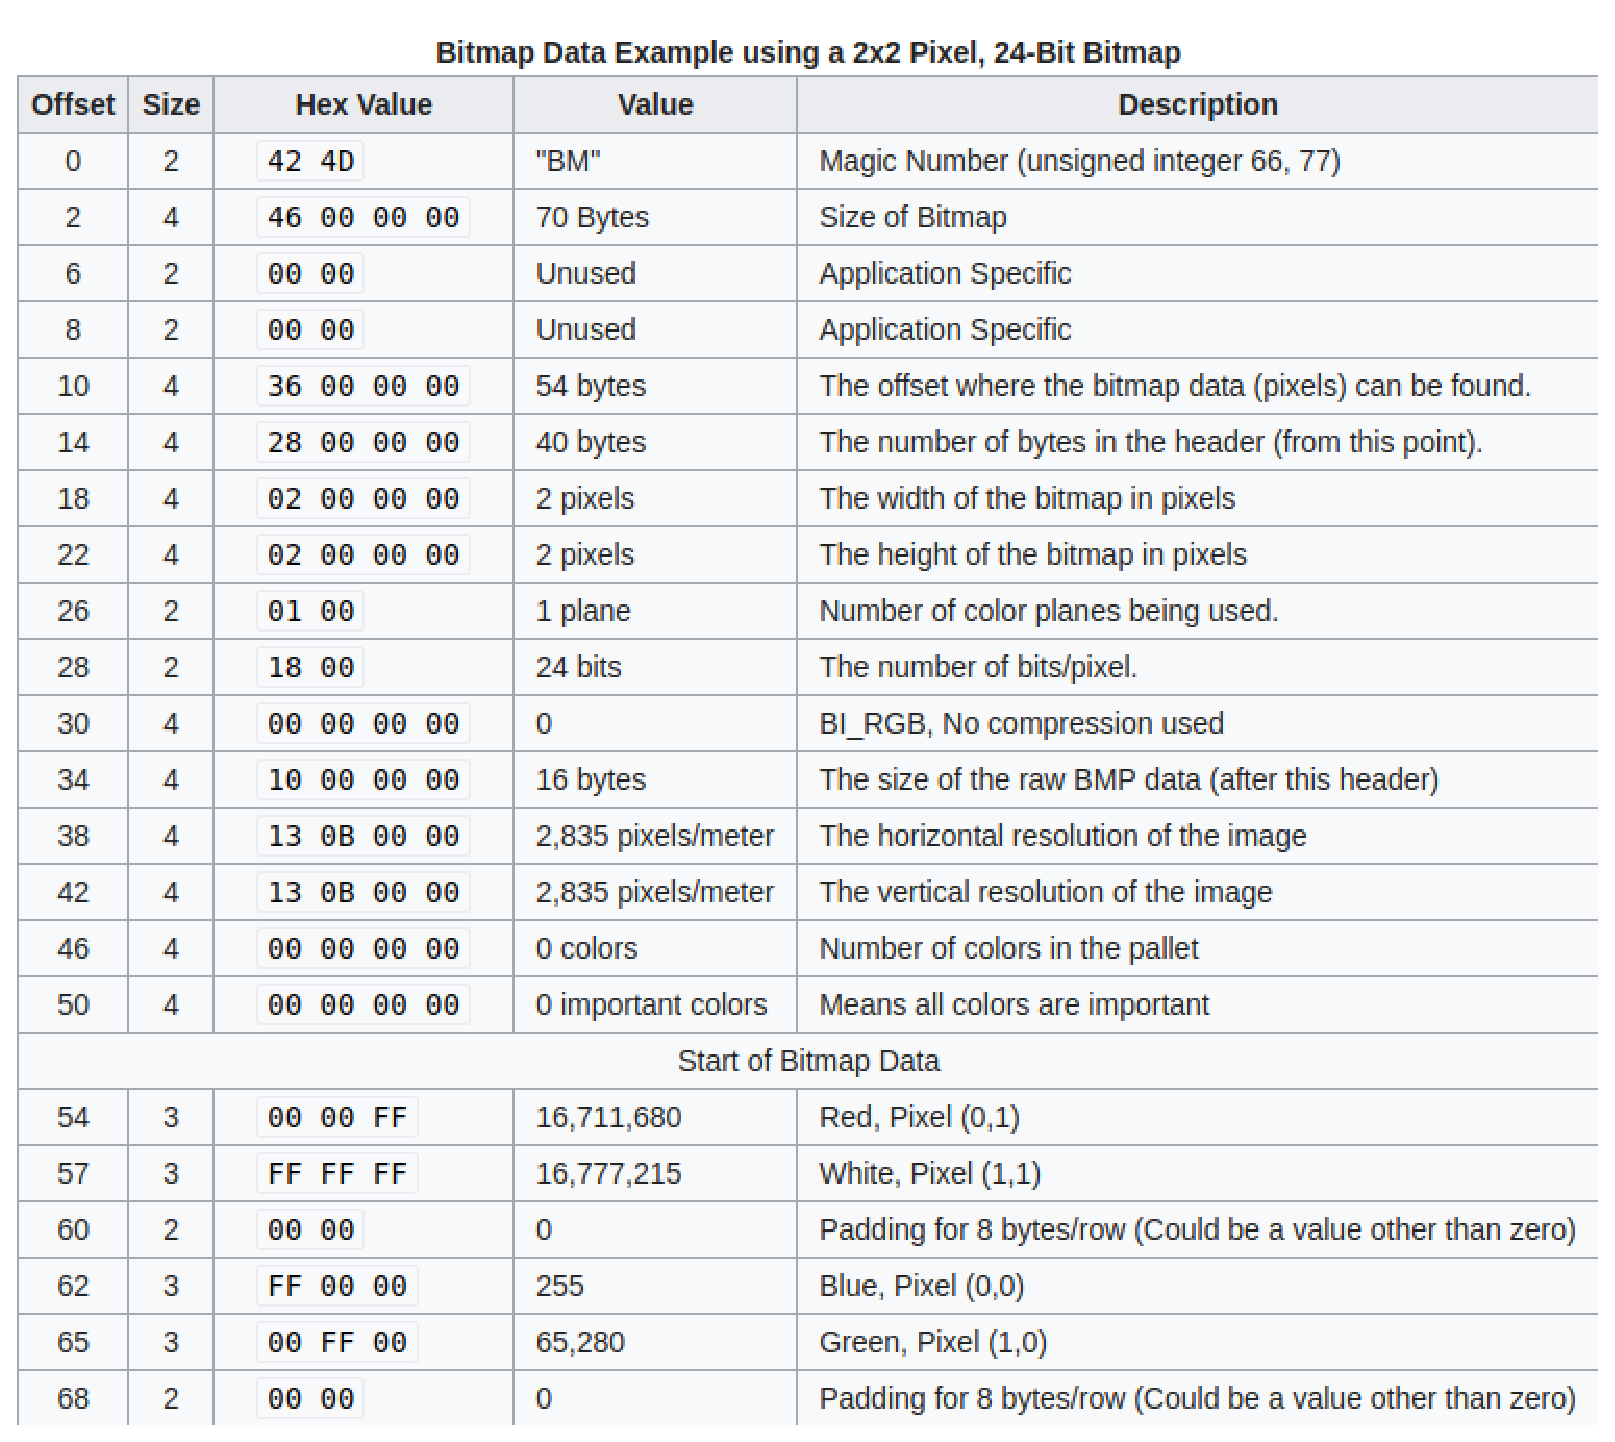
\includegraphics[width=15cm]{bitmap_structure.eps}\\\\

\subsection{Application du LSB}
Nous avons choisi de cacher des informations à partir de la fin du header c'est-à-dire après le cinquante-quatrième byte du fichier.
Cela nous permet d'amoindrir les altérations de l'image en sortie car les modifications sont invisbles à l'oeil humain.
De plus, comme dit plus haut, ce fichier n'utilisant généralement jamais d'algorithme de compression, il ne nous sera pas nécessaire
de nous soucier de perte de données qui impacteraient le décodage d'une image dans laquelle on aurait caché des données.

\vspace{1.5cm}

\begin{figure}[H]
    \centering
    \subcaptionbox{Bitmap source}{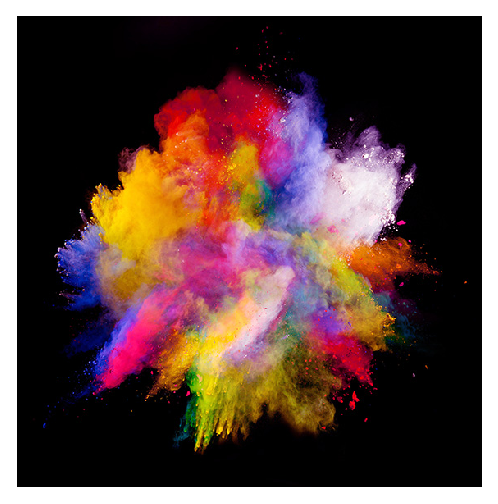
\includegraphics[width=0.45\textwidth]{splash_color_src.eps}}%
    \hfill
    \subcaptionbox{Bitmap dest }{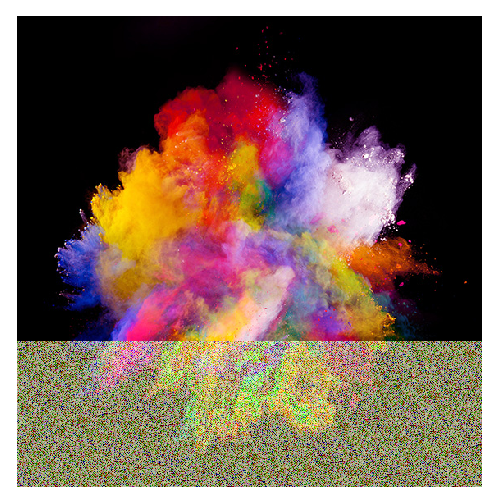
\includegraphics[width=0.45\textwidth]{splash_color_dest.eps}}%
    \caption{Encodage d'un fichier texte dans un bitmap}
\end{figure}